\scanpage{66}
\mspage{65}
% E: deletion|upper left crossed through by diagonal strokes|sont en est qu'elles
\deleted{\deleted{\unsure{sont}} \unsure{en est qu'elles|ceux desquels} \unsure{il y a} une application canonique de la surface recollée dans $X$! \deleted{Si on recolle $b$ à $a$} \inserted{Non, c'est vrai pour $a'$}, \deleted{donc} \unsure{car}, pour $\alpha$ choisi, on choisira l'identification.}
% E: text|left upper middle|Si on veut une application naturelle
Si on veut une application naturelle de la surface recollée dans $X$, qui sur $\Delta_D$, $\Delta_{D'}$ se réduise au plongement canonique, il faut \inserted{(semble-t-il)} que $b$ et $\alpha$ se réalisent par le $=$ segment plongé dans $X$, ce qui \inserted{semble} imposer $\alpha=a'$. Mais si on convient de remplacer $\Delta_D$ par un disque \unsure{un plus petit|un peu petit} $\Delta_D^*$ \inserted{dont le bord} passe par $s$ (cf pointillé ci-contre), et déplacer \unsure{canoniquement} $b$ en $b^*$, et faire le recollement le long de $b^*$ plutôt que $b$, \deleted{donc} et pareil pour le disque $\Delta_{D'}$, (de façon à faire coïncider les images de $a$ et $a'$ dans $X$), on voit qu'on arrive à \deleted{\unsure{faire appliquer}} \inserted{\unsure{trouver}} une application de la surface recollée dans $X$, même en choisissant $\alpha=a$.
% E: drawing|lower left in paragraph|Delta_D star s b star
\figure{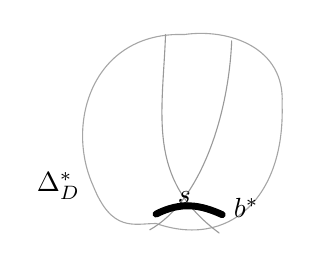
\begin{tikzpicture}[x=.8cm,y=.8cm,line cap=round]
\draw[gray!70] (0,1.8) .. controls (-1.45,1.85) and (-1.9,.4) .. (-1.45,-.6) .. controls (-1.15,-1.35) and (-.8,-1.2) .. (-.45,-1.2) .. controls (.7,-1.6) and (1.6,-.8) .. (1.55,.7) .. controls (1.6,1.6) and (.7,1.9) .. (0,1.8);
\draw[gray!80] (-.3,1.8) .. controls (-.35,.5) and (-.6,-.5) .. (.55,-1.35);
\draw[gray!80] (.75,1.7) .. controls (.7,.5) and (.25,-.85) .. (-.55,-1.3);
\draw[line width=2.5pt] (-.45,-1.05) .. controls (-.05,-.85) and (.25,-.9) .. (.6,-1.06);
\node at (0,-.78) {$s$};\node[right] at (.63,-.95) {$b^*$};\node at (-2,-.6) {$\Delta_D^*$};
\end{tikzpicture}}
% E: text|bottom left continuing top right|Le choix le plus naturel quand même
Le choix le plus naturel quand même (\deleted{\unsure{dans}} pt de vue application dans $X$), semblerait $\alpha=a'$. \unsure{Donc|Dans}, sur le terrain de dessin --- \uline{continuation} d'une rive par la suivante --- l'application $\mathcal X\longrightarrow X$ est une \uline{``immersion''}.
% E: drawing|right upper middle|two crossing orange arcs orientation arrows
\figure{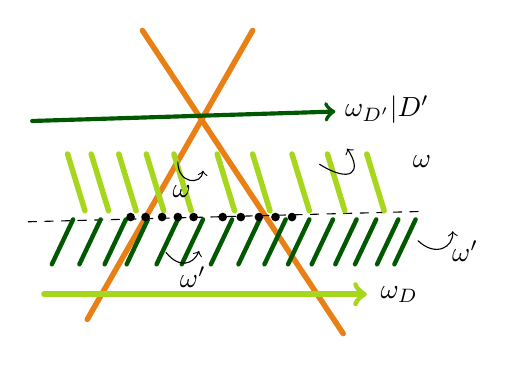
\begin{tikzpicture}[x=1cm,y=1cm,line cap=round,line join=round]
\draw[orange!65!brown,line width=2pt] (-1.3,2.15)--(1.25,-1.7);
\draw[orange!65!brown,line width=2pt] (.1,2.15)--(-2,-1.52);
\draw[green!35!black,line width=1.5pt,->] (-2.7,1)--(1.15,1.12);
\draw[yellow!65!green,line width=2pt,->] (-2.55,-1.2)--(1.55,-1.2);
\node[right] at (1.6,-1.2) {$\omega_D$};
\node[right] at (1.15,1.14) {$\unsure{\omega_{D'}|D'}$};
\draw[dashed] (-2.75,-.28)--(2.2,-.15);
\foreach \x in {-2.25,-1.95,-1.6,-1.25,-.9,-.35,.1,.6,1.05,1.55}{\draw[yellow!65!green,line width=2pt] (\x,.58)--(\x+.22,-.14);}
\foreach \x in {-2.45,-2.1,-1.78,-1.5,-1.12,-.8,-.43,-.08,.25,.55,.85,1.15,1.4,1.68,1.9}{\draw[green!35!black,line width=1.6pt] (\x,-.82)--(\x+.27,-.25);}
\foreach \x in {-1.45,-1.26,-1.05,-.85,-.65,-.28,-.05,.18,.39,.6}{\fill (\x,-.22) circle (.055);}
\draw[->] (-.85,.48) .. controls (-.85,.2) and (-.55,.18) .. (-.53,.37);\node at (-.8,.1) {$\omega$};
\draw[->] (.95,.45) .. controls (1.35,.2) and (1.5,.35) .. (1.3,.65);\node at (2.25,.48) {$\omega$};
\draw[->] (-1,-.67) .. controls (-.83,-.88) and (-.65,-.82) .. (-.58,-.65);\node at (-.66,-.98) {$\omega'$};
\draw[->] (2.2,-.52) .. controls (2.42,-.73) and (2.65,-.61) .. (2.64,-.4);\node at (2.8,-.65) {$\omega'$};
\end{tikzpicture}}
% E: text|right lower half|Dans cette optique la rive de D'
Dans cette optique \inserted{\unsure{donc}}, la rive de $D'$ i.e. l'arc sur $\partial\Delta_{D'}$ qui exprime l'orientation de \deleted{\unsure{spécialisation}} \inserted{\unsure{générisation}} vers $D$ est $a'$ --- i.e. celle qui ``fait face'' à la rive $a$, et non $a$ qui en est déduit par ``transport parallèle'' au cours de la déformation de spécialisation $D\longrightarrow D'$. Ce choix semble parfaitement naturel --- l'inverse,
